The advantages of content-based superpixels are shown in several important vision tasks.

\subsection{Classification}

An AlexNet classifier trained on ImageNet data \cite{alex2012net} was used to classify images in the COCO dataset \cite{coco14data}. The superpixel centers were sampled from a Gaussian mixture centered at each region of interest (ROI) with equal proportions, while allocating $10\%$ of samples to background.

\begin{figure}[h]
	\centering
	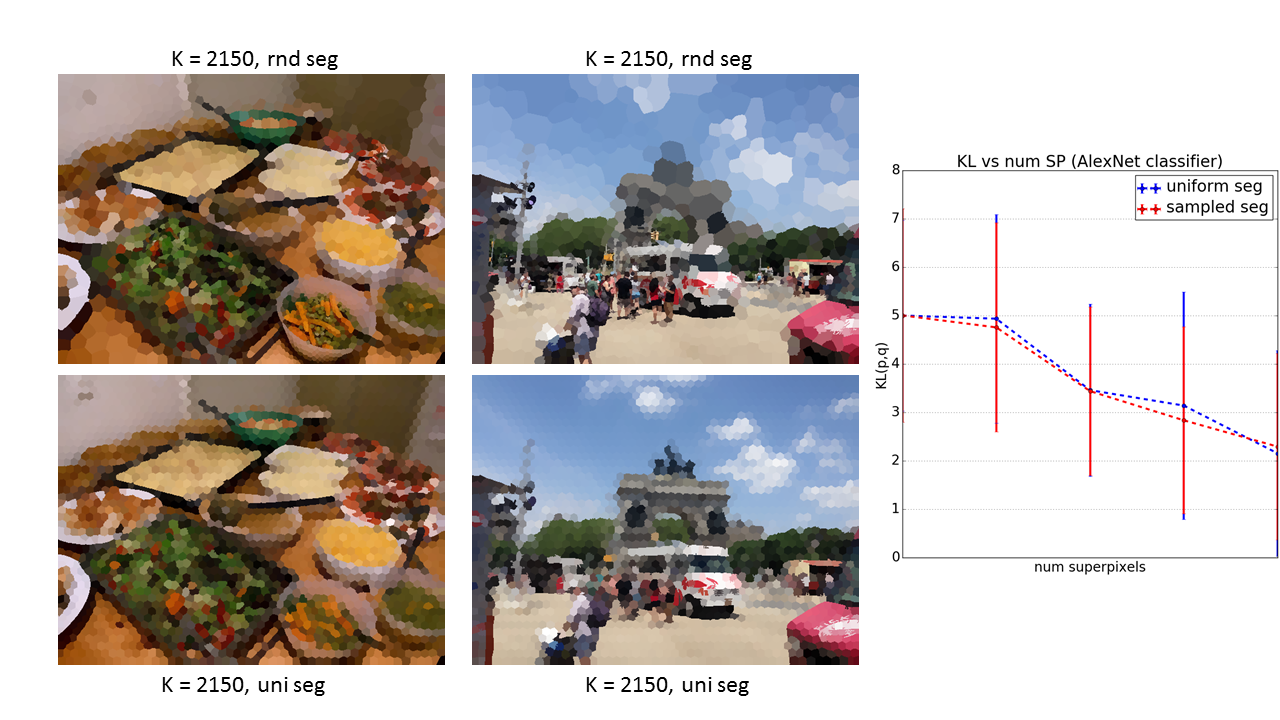
\includegraphics[width=0.8\textwidth, trim={10 10 10 10}]{figures/coco_merged.png}
	\caption{Top-row: content-based superpixels. Bottom-row: uniform superpixels. Right: KL divergence between classifier outputs.}
    \label{fig:coco}
\end{figure}

Figure \ref{fig:coco} shows the difference between content-based (top row) and uniform (bottom row) superpixels for sample images from the COCO dataset \cite{coco14data}. Also, shown on the right is the KL divergence of the output of AlexNex classifier in the two cases. We can see that the content-based superpixels are slightly lower compared to unifom superpixels.


